\documentclass{beamer}
\usepackage[utf8]{inputenc}
\usepackage{xeCJK} 
\usepackage[T1]{fontenc}
\usepackage{mathabx}
\usepackage{amsmath} 
\usepackage{mathpazo}
\usepackage{bibentry}
\usepackage{tikz}
\usepackage{caption}
\usepackage{graphicx, subfig}

\usetikzlibrary{scopes}
\def\iangle{35} % Angle of the inclined plane
\def\down{-90}
\def\arcr{0.5cm} % Radius of the arc used to indicate angles

\usetheme{Boadilla}
\usecolortheme{wolverine}
\useoutertheme{miniframes}

\title{VP160 Recitation Class IV}
\subtitle{Non-inertial FoR}
\author{Zeyi Ren}
\institute{UM-SJTU Joint Institute}

\begin{document}

\maketitle

%\frame{\tableofcontents}

\section{Non-inertial FoR}
\begin{frame}
  \begin{block}{Recall}
    The non-inertial FoR is a frame of reference that is not in a linear motion with uniform velocity relative to an inertial frame of reference.
  \end{block}
  \pause
  \textcolor{blue}{Basic Formula}
  $$
  \vec{a^{\prime}}=\vec{a}-\vec{a_{O}^{\prime}}-\frac{d \vec{\omega}}{d t} \times \vec{r^{\prime}}-2(\vec{\omega} \times \vec{v^{\prime}})-\vec{\omega} \times(\vec{\omega} \times \vec{r^{\prime}})
  $$
  \pause
  $$
  m \vec{a^{\prime}}=\vec{F}-m \vec{a_{O}^{\prime}}-m \frac{d \vec{\omega}}{d t} \times \vec{r^{\prime}}-2 m(\vec{\omega} \times \vec{v^{\prime}})-m \vec{\omega} \times(\vec{\omega} \times \vec{r^{\prime}})
  $$
  \pause
  How to derive the formula?
\end{frame}

\begin{frame}
  \begin{block}{Recall}
    Newton's Second Law doesn't hold in non-inertial FoR. To describe the motion in non-inertial FoR, we need to add the forces of inertia (pseudo-forces) into "Newton's Second Law" in non-inertial FoR.
  \end{block}
  \pause
  Add $\mathbf{F_{Unreal}}$:
  $$
  \mathbf{F'} = \mathbf{F_{Real}} + \mathbf{F_{Unreal}}
  $$
  \pause
  to maintain the "Newton's Second Law" in non-inertial FoR:
  $$
  \mathbf{F'} = m \mathbf{a'}
  $$
  \pause
  $$
  \mathbf{F_{Unreal}} = -m \vec{a_{O}^{\prime}}-m \frac{d \vec{\omega}}{d t} \times \vec{r^{\prime}}-2 m(\vec{\omega} \times \vec{v^{\prime}})-m \vec{\omega} \times(\vec{\omega} \times \vec{r^{\prime}})
  $$
\end{frame}

\begin{frame}{Drift ``Force'' $-m\vec{a_{O'}}$}  
\begin{figure}[H]
\centering
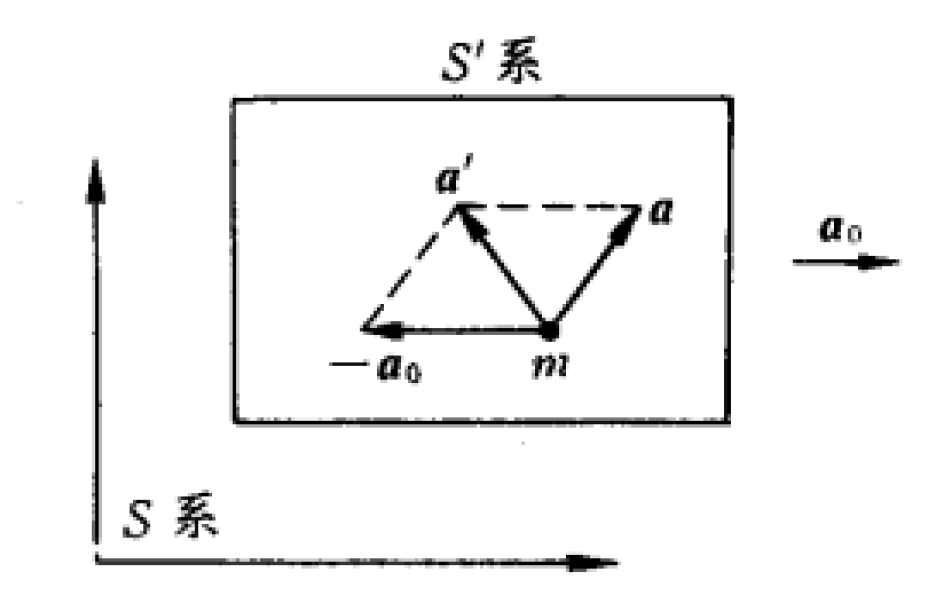
\includegraphics[width=0.35 \linewidth, angle =0]{drift.png}
% \begin{center}
%   Figure 1: Drift ``Force''.
% \end{center}
\label{fig:1}
\end{figure}
\pause
Newton's Second Law in inertia FoR $S$: 
$$\mathbf{F}=m\mathbf{a}$$\pause
Acceleration in non-inertial FoR $S'$:
$$\mathbf{a'} = \mathbf{a}+(-\mathbf{a_0})$$\pause
$$\Rightarrow \mathbf{F'}= m\mathbf{a'}=m\mathbf{a}+m(-\mathbf{a_0})=\mathbf{F}+m(-\mathbf{a_0})$$
\end{frame}

\begin{frame}{Centrifugal ``Force'' $-m\vec{\omega}\times(\vec{\omega}\times \vec{r'})$}
  \begin{figure}[htbp]
  \centering
  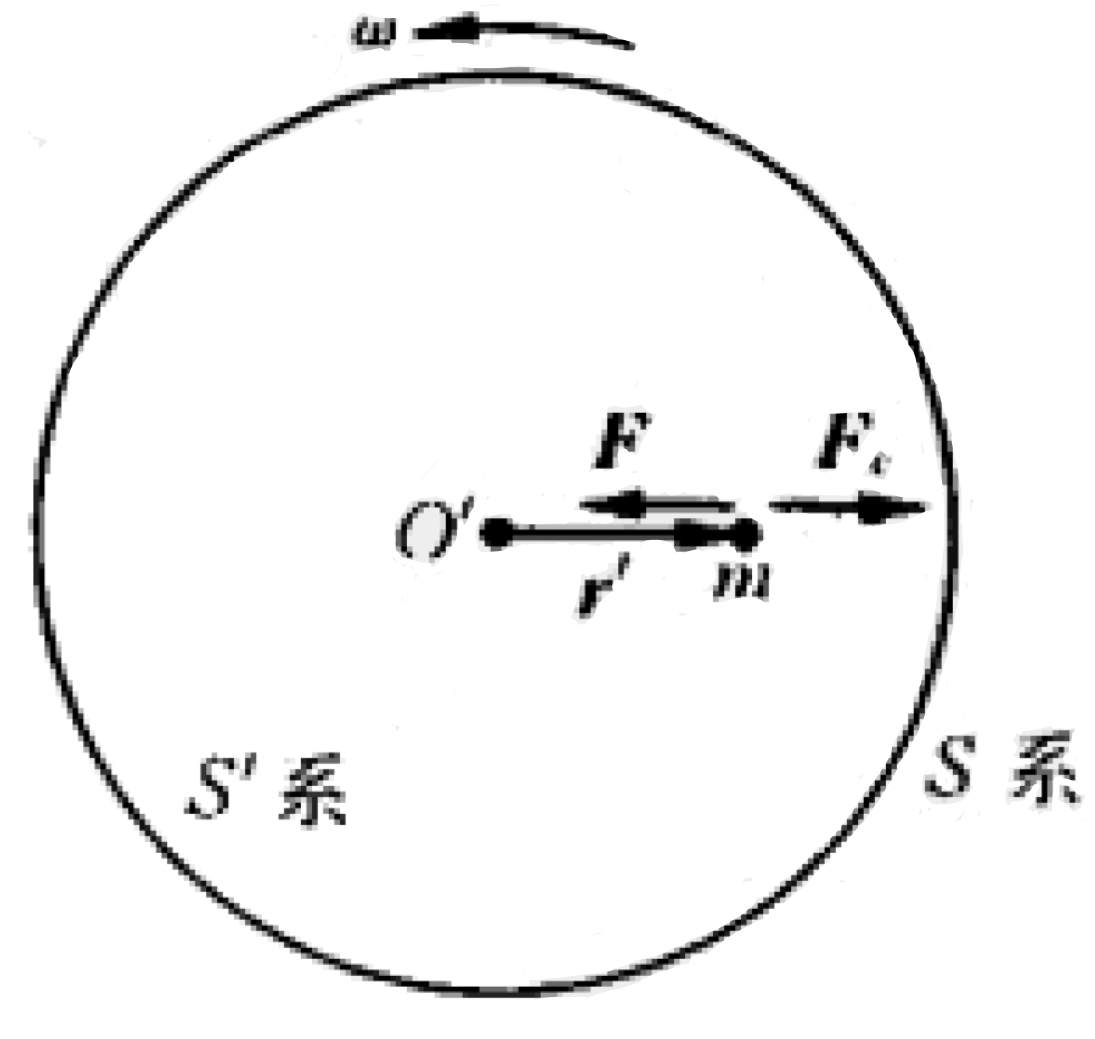
\includegraphics[width=0.25 \linewidth, angle =0]{centrifugal.png}
  % \begin{center}
  %   Figure 2: Centrifugal ``Force''.
  % \end{center}
  \label{fig:2}
  \end{figure}\pause
  Uniform circular motion in $S:$
  $$
  \mathbf{a}=-\omega^2\mathbf{r'},\quad \mathbf{F} = m\mathbf{a}=-m\omega^2\mathbf{r'}
  $$\pause
  In $S'$:
  $$\mathbf{a'}=0,\quad \mathbf{F'}=m\mathbf{a'}=0$$\pause
  Thus, we need
  $$\mathbf{F_c}=m\omega^2\mathbf{r'}\quad\text{s.t.}\quad \mathbf{F'}=\mathbf{F}+\mathbf{F_c}=0$$
\end{frame}

\begin{frame}{Coriolis ``Force'' $-2 m(\vec{\omega} \times \vec{v^{\prime}})$}
  \begin{figure}[htbp]
  \centering
  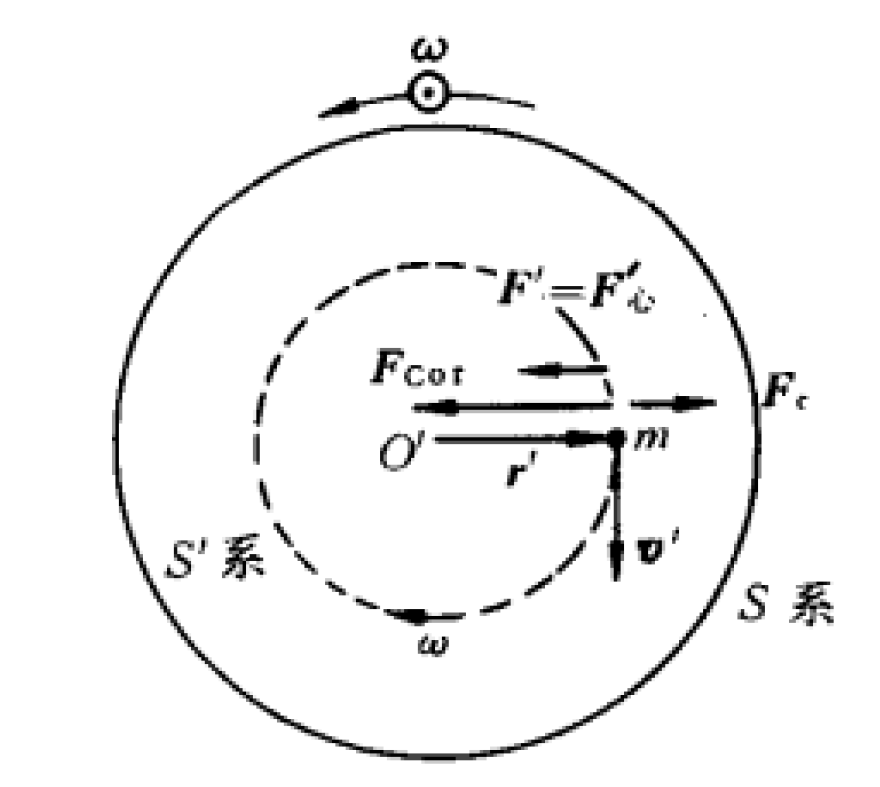
\includegraphics[width=0.23 \linewidth, angle =0]{coriolis.png}
  % \begin{center}
  % Figure 3: Coriolis ``Force''.
  % \end{center}
  \label{fig:3}
  \end{figure}\pause
  $m$ stays still in $S$:
  $$\mathbf{F} = 0$$\pause
  $m$ moves in a uniform circular motion in $S'$:
  $$\mathbf{a'}=-\omega^2\mathbf{r'},\quad \mathbf{F'}=m\mathbf{a'}=-m\omega^2\mathbf{r'}$$\pause
  Thus, we need (Don't forget the centrifugal force we added)
  \begin{align*}
  \mathbf{F_{Cor}}=-2m\omega^2\mathbf{r'}\quad\text{s.t.}\quad \mathbf{F'}=\mathbf{F}+\mathbf{F_c}+\mathbf{F_{Cor}} & =0+m\omega^2\mathbf{r'}+(-2m\omega^2\mathbf{r'})\\ &=m\mathbf{a'} 
  \end{align*}
\end{frame}

\begin{frame}{Euler "force" $-m \frac{d \vec{\omega}}{d t} \times \vec{r^{\prime}}$}
  \begin{itemize}
    \item Need to be considered when $\omega$ is time-variant.\pause
    \item Also called Tangential inertial forces.\pause
    \item Conventionally, we use $\vec{\beta}$ to denote the angular acceleration $\frac{d \vec{\omega}}{d t}$.
  \end{itemize}
\end{frame}

\section{Exercise}
\begin{frame}
\textcolor{blue}{Exercise 1}

A particle with mass $m$ is inside a pipe that rotates with constant
angular velocity $\omega$ about an axis perpendicular to the pipe.The
kinetic coefficient of friction is equal to $\mu_k$. Write down (do not
solve!) the equation of motion for this particle in the non-inertial
frame of reference of the rotating pipe. There is no gravitational
force in this problem.
\begin{figure}[htbp]
\centering
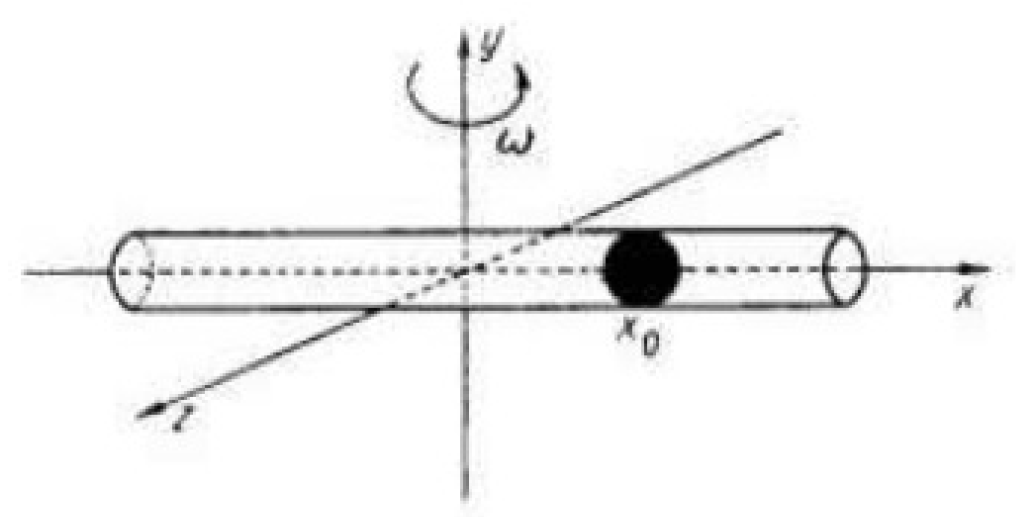
\includegraphics[width=0.5 \linewidth, angle =0]{ex1.png}
% \caption{.}
\label{fig:4}
\end{figure}
\end{frame}

\begin{frame}
\textcolor{blue}{Exercise 2}

If we let go an object $100m$ above the equator. Ignore the air
drag, calculate the deviation caused by Coriolis Force.
\end{frame}


\begin{frame}{Reference}
  \begin{thebibliography}{9}
  \setbeamertemplate{bibliography item}[article]
  \bibitem{C} Yigao Fang.\\
  \textcolor{black}{VP160 Recitation Slides.}\\
  2020
  \bibitem{C} Haoyang Zhang.\\
  \textcolor{black}{VP160 Recitation Slides.}\\
  2020
  \setbeamertemplate{bibliography item}[book]
  \bibitem{C} Yousheng Shu (舒幼生).\\
  \textcolor{black}{\textit{Mechanics (力学)}}\\
  Peking University Press, 2005
  % \setbeamertemplate{bibliography item}[book]
  % \bibitem{C} Jiafu Cheng (程稼夫).\\
  % \textcolor{black}{\textit{中学奥林匹克竞赛物理教程:力学篇}}\\
  % University of Science and Technology Press, 2013
  \end{thebibliography}
  \end{frame}
  \end{document}



